As explained in the chapter \ref{sec:The_Decay_Equation} in this thesis we are considering the decay of 3 isotopes, where the $A$ matrix is of the form equation (\ref{eq:A_matrix}). In this case, we have an analytical solution for our problem and this solution is given by the set of equations (\ref{eq:analytical_sol}).

Following the idea introduced in chapter \ref{sec:PINNs}, we start to solve our problem writing a supervised NNs.\\
We do this to better understand the problem that we want to solve, but also because training a supervised NN will be a benchmark for us to understand if it is possible to solve this problem using a neural network and if so if the architecture that we are using is sufficient to learn the problem. This is because if also this network is failing then will also the PINN.

The core part of this NN is the loss function. To train the network we decide on a time $t$ and divide it into $t_{step}$ steps. These will be inputs of the network and we will evaluate the NN at each of them. To optimize the parameter of the network we will use the gradient descent method minimizing the outputs of $\Phi$ at all the time steps with the respective analytical solution computed using equation \ref{eq: analytical_sol} at all the time steps.
%%%%%%%%%%%%%%%%%%%%%%%%%%%%%%%%%%%%%%%%%
%FIGURA 
\begin{figure}
\centering
    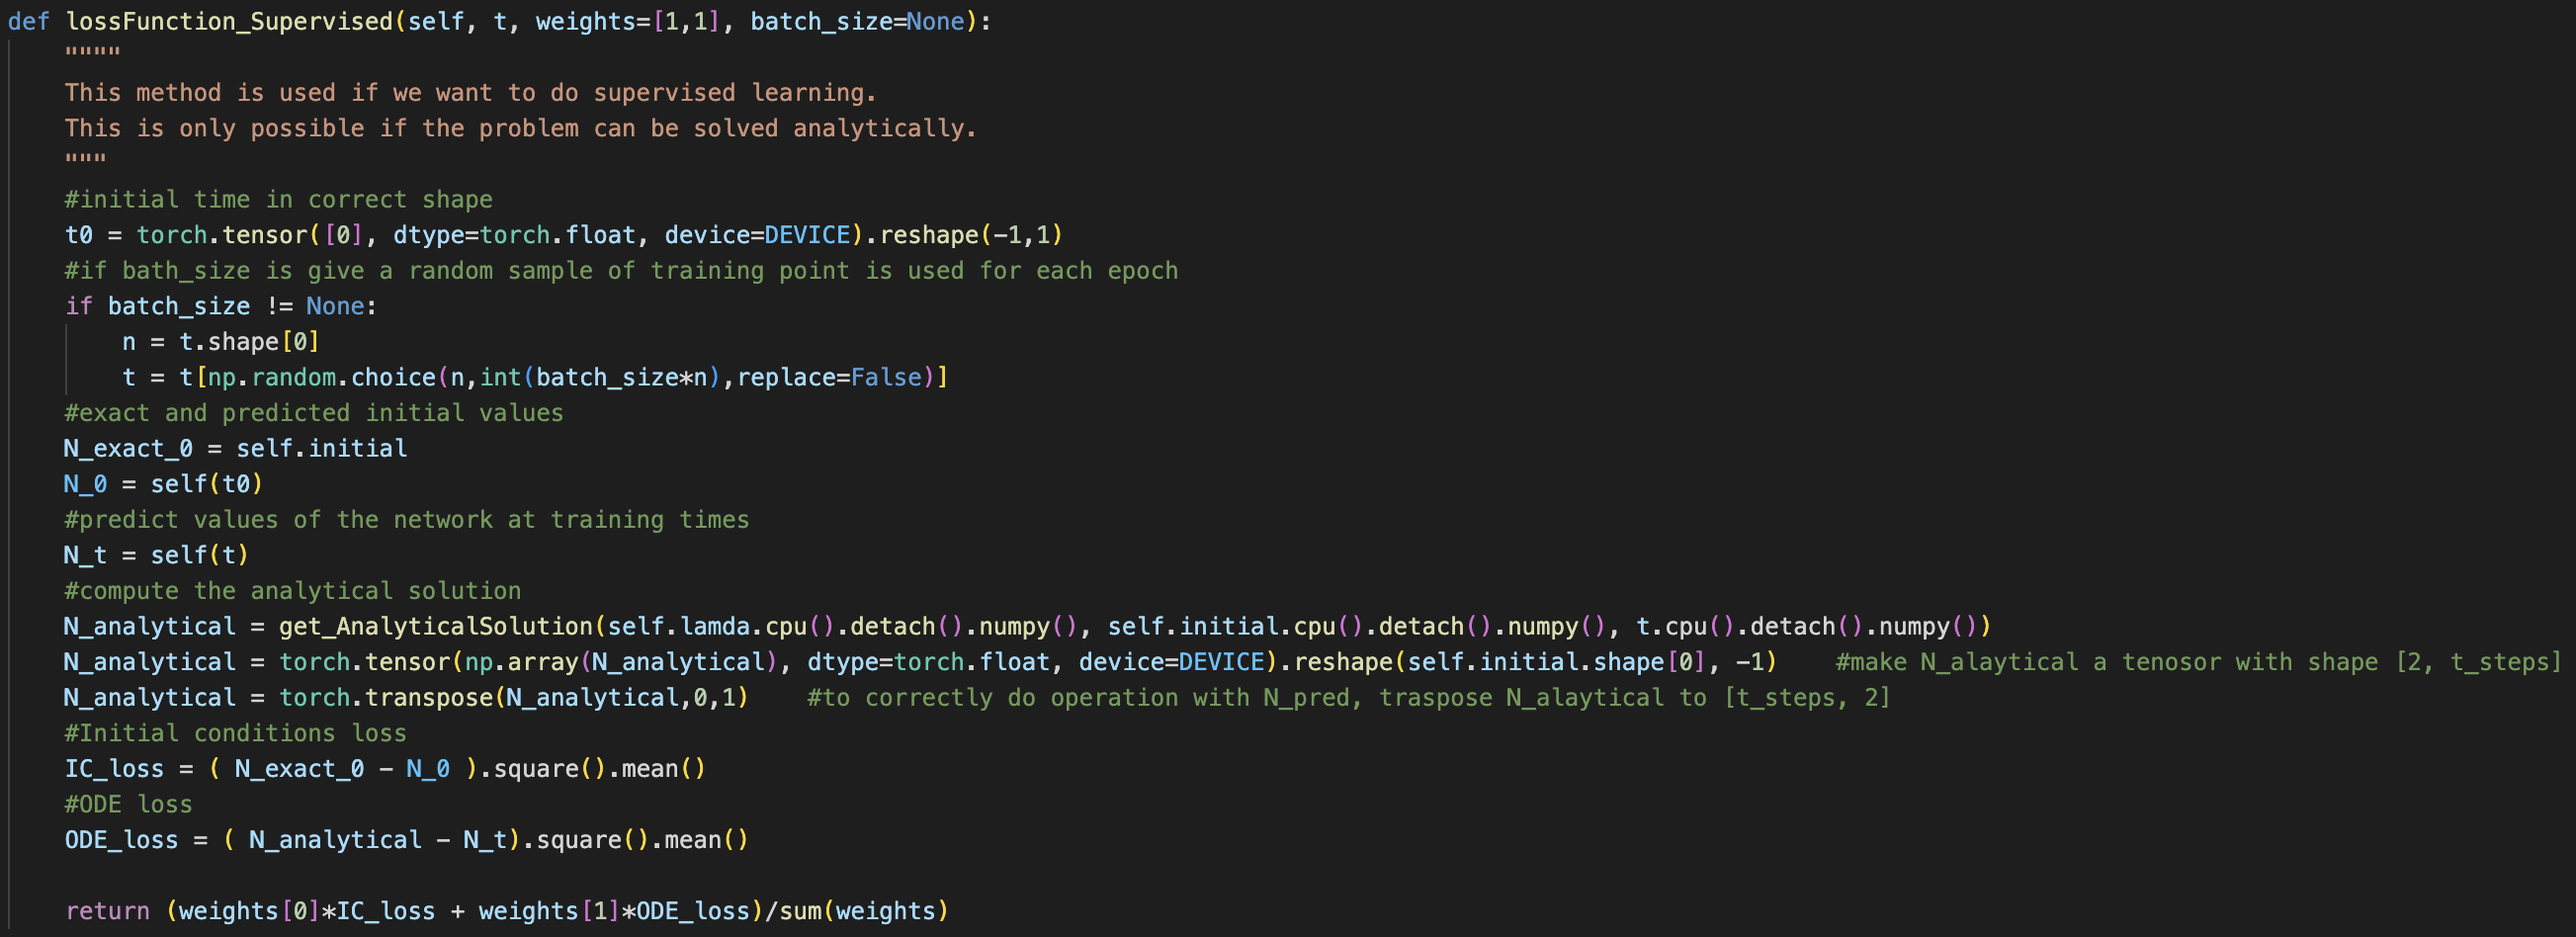
\includegraphics[width=0.90\linewidth]{figures/02.1 Analytical Solution/Loss_function_Supervised.png}
    \caption{Il grafico mostra la sezione d'urto dei processi dominanti previsti dallo SM per collisioni tra elettroni-positroni non polarizzati ed il numero di eventi previsto per una luminosità integrata di $5.6\, \text{ab}^{-1}$ in funzione dell'energia del centro di massa $\sqrt{s}$. A $240$ GeV si può osservare in rosso il picco della sezione d'urto per il processo Higgs-Strahlung ($e^{+}e^{+} \rightarrow ZH$).}
    \label{fig:cross section}
\end{figure}
%%%%%%%%%%%%%%%%%%%%%%%%%%%%%%%%%%%%%%%%%
% \begin{lstlisting}[frame=single]
%     def lossFunction_Supervised(self, t, weights=[1,1], 
%                                 batch_size=None):

%     #initial time in correct shape
%     t0 = torch.tensor([0], dtype=torch.float,
%                         device=DEVICE).reshape(-1,1)
%     #if bath_size is give a random sample of training point
%     #is used for each epoch
%     if batch_size != None:
%         n = t.shape[0]
%         t = t[np.random.choice(n,int(batch_size*n),
%                                 replace=False)]
%     #exact and predicted initial values
%     N_exact_0 = self.initial
%     N_0 = self(t0)
%     #predict values of the network at training times
%     N_t = self(t)
%     #compute the analytical solution
%     N_analytical = get_AnalyticalSolution(
%                         self.lamda.cpu().detach().numpy(),
%                         self.initial.cpu().detach().numpy(),
%                         t.cpu().detach().numpy())
%     N_analytical = torch.tensor(np.array(N_analytical),
%                                 dtype=torch.float,
%                                 device=DEVICE).reshape(self.initial.shape[0], -1)
%     N_analytical = torch.transpose(N_analytical,0,1)    #to correctly do operation with N_pred, traspose N_alaytical to [t_steps, 2]
%     #Initial conditions loss 
%     IC_loss = ( N_exact_0 - N_0 ).square().mean()
%     #ODE loss
%     ODE_loss = ( N_analytical - N_t).square().mean()

%     return (weights[0]*IC_loss + weights[1]*ODE_loss)/sum(weights)
% \end{lstlisting}